\documentclass[12pt]{article}
\usepackage{graphicx}
\DeclareGraphicsExtensions{.pdf,.png,.jpg}

\title{Scalable\\ Data Integration and Entity Resolution\\in Hadoop}

\author{Eric Peyton\\
\small Georgia Institute of Technology\\
\small CS 4365 Project\\
}

\begin{document}
\maketitle

\begin{abstract}
Data integration is the process of combining multiple data sources through an ETL procedure into a common unified view of the data. Integrating large datasets introduces a number of new challenges, especially if much of the data is noisy. These heterogenous data sources are manipulated to fit the common schema and loaded. Entity resolution is the process of resolving duplicated entities and relationships between them. This process may involve complex matching algorithms and machine learning.

I am proposing a Java framework to extend the Apache Hadoop library and facilitate smooth parallel data integration and entity resolution on a cluster. Hadoop provides a powerful platform for parallel computing. However, often many adjustments to an application are required in order to fit the MapReduce programming model. This typically involves much code and testing. For integrating data, this includes writing a custom MapReduce job for every new data source. To resolve entity duplicates, more MapReduce jobs have to written to match, unify, and merge the duplicate entities. The proposed Java framework will greatly simpifly this process and provide robust tools for integrating large data sources and deduplicating the results.
\end{abstract}
\section{Problems Addressed}
In the ``big data'' of today, information about real-world entities often comes from large, diverse, and unstructured sources. \\\\
For example,  we can examine the case of constructing information about real-world events in a city (e.g. a concert, wine-tasting, or festival). 
There is no central or complete source for gathering information about these on-goings. Many are user-submitted through Facebook, others found through ticketing websites, or some may even appear only in the website of a local magazine. 
This data may come in structured or unstructured formats and grows daily among hundreds of cities. 
Since events often appear in multiple sources, the number of event records to organize can easily scale into millions a year. 
The same problem can be extended to different entity types, such as local businesses or human information.\\\\
Scalable techonology is needed to integrate and disambiguate these records into representations of real-world of entities. However, the underlying process for this remains similar across domains and types of entities, such that repetitive work is done for each new entity type. This issue is amplified when a big data platform such as Hadoop requires verbose Java code for MapReduce jobs. A unified and systematic approach to solving the problem would prevent redundant efforts.

\section{Objectives}
In order to address these problems, I created a framework to translate the problems of heterogenous data integration and entity resolution to the MapReduce programming model on the Hadoop platform. \\\\
To limit the scope of the project, I intended to focus on distributed data integration into a record-matching entity resolution framework. 
In my project, resolving entities involves matching them, clustering them on transitive relationships, and computing a single representation of a cluster. 
In addition, this process will be completed with a global schema and schema mappings provided by the user.\\\\
Another objective was to create a generic and unified solution to solve these problems across multiple domains.
In order to accomplish this, I treated the functions for schema-mapping, and matching, and merging as black-boxes that are provided by a user of the framework. These simple functions help reduce boilerplate code associated with MapReduce jobs and encourage (relatively) concise code to describe the relationships between entities.\\\\
Lastly, this project is intended as a tool for other programmers. 
Implementation of the framework and black-boxes are completely in Java, and there is no GUI component for management by non-technical users. 
This eases integration with Hadoop MapReduce and provides all the logical functionality of Java to users. 

\section{Approach}
This framework is built upon the Hadoop platform and the MapReduce batch-processing programming model. 
Hadoop was chosen for its easy and low-cost scaling abilities, and its popularity among big-data platforms.\\\\
The data integration and entity resolution process consists of five component jobs: the importers, builder, grouper, combiner, and exporter.
\subsection{Importers}
An importer job is created for each new data source. The framework utilizes both built-in and custom MapReduce input formats for importing data from HDFS into the job. Currently, the project supports JSON, XML, text, and CSV data inputs to an import job. In the importer, each data source is mapped to a global schema using a block-box function that is unique to the data source. Changes in a data source require subsequent changes to its mapping function.\\\\
In the mapper of the importer, an input record is mapped to a serializable Java POJO using automatic and user-provided conversions. These records are then distributed across the cluster to a number of reducers. The reducer machines map the record input schema to the global schema and write the output to an intermediate location on HDFS.\\\\
Additionally, the black-box functions allow for normalization, validation, and data cleaning during the import stage.
\subsection{Builder}
The builder handles the matching component of the entity resolution process.\\\\
A simple pairwise comparison of every single entity requires $O(n^2)$ comparisons, thus is very inefficient for a large number of records. An improvement to pairwise comparison, called ``blocking'', is implemented within the mapper component of the builder.
\subsection{Grouper}
\subsection{Combiner}
\subsection{Exporter}


%\begin{figure}
%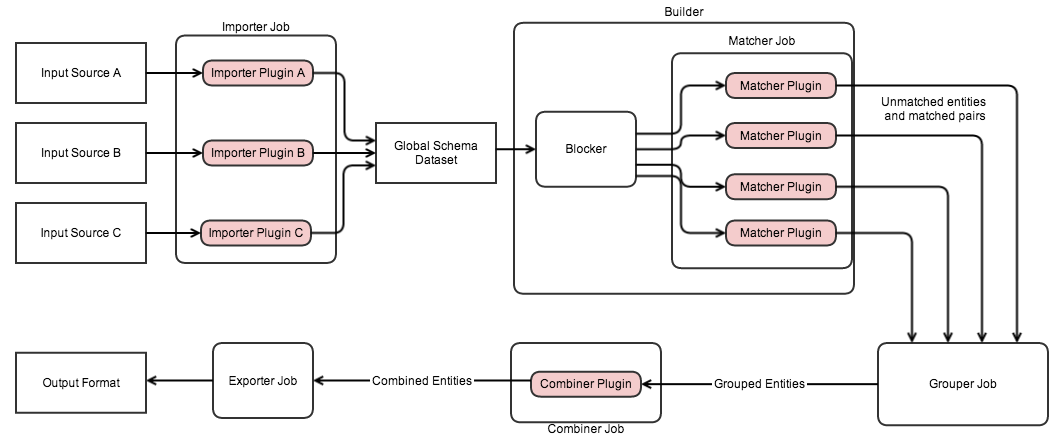
\includegraphics[scale=.5]{architecture}
%\end{figure}

First, a large dataset is converted into a set of common entities.
In this first stage, a dataset is fed into the normalizing stage, which is a MapReduce job in Java. Hadoop jobs already support many different file formats as inputs, and the framework will support them as well. Instead of extending the typical Runner/Mapper/Java classes for a job, the user will extend a class in the framework. In this subclass, the user will only need to define the relationship between the input data and the entity without writing redundant MapReduce boilerplate code.

In the second stage, all the entities generated in the first stage are pushed by the framework to the entity store in HBase. No deduplication or matching occurs at this stage, so the entity store may contain duplicates until the third stage. For particurlarly large datasets, the entity store may contain sparse data.

Finally, the entity store in HBase provides the input for the merging MapReduce job. Here, entities are matched together based on key attributes that are specified by the user. This may include fuzzy matching. The matched entities are referenced together in the reference table in HBase.

To utilize the framework, a user will include the framework Jar into their application. Then they will create a Java class to define the common entity. Java classes will be extended to provide infromation about each data source, entity relationships, and matching logic. Next, via a command on a Hadoop server, the framework will create the required infrastructure. Another command will integrate a specified source. A last command will merge, match, and provide the user with a unified output in a file.

\section{Architecture}

\section{Lessons Learned}

\section{Future Work}





\end{document}
